\chapter{Science Is Elementary 1}

% \begin{figure}[H]
%     \centering
%     \includegraphics[width=\textwidth/2]{./Games/EveryChildCanSucceed/Images/EveryChildCanSucceed7CD.png}
%     \caption{Every Child Can Succeed 7 CD}
% \end{figure}

The first of the Science Is Elementary games published and released by The Lightspan Partnership for the PlayStation 1.

Science Is Elementary 1 features four video programs:

\begin{itemize}
    \item Let's Explore Plants
    \item Let's Explore Animals
    \item Let's Explore Sound
    \item Let's Explore Light and Shadows
\end{itemize}

\clearpage
\newpage

\section{Let's Explore Plants}

\subsection{Audio Summary}

In "Let's Explore Plants", we investigate the shapes and sizes of the leaf, root and stem parts of plants. We also discuss plant usefulness and the function of seeds. In the exploration, we look at the effects of air, light and water on plant growth.

\subsection{Transcription}

Young Girl: Plants are everywhere. What do all these plants look like? People and animals use plants. How are these plants being used in these scenes?

Young Girl (voice over): Time for a true story about how one special man planted many seeds that would make more of themselves. Long ago, a man named John Chapman lived in Massachusetts where there were many apple orchards. He enjoyed apples and the orchards so much. From his home, he could see pioneer wagons on their way to a new land in the Ohio Valley. He learned that these pioneers had to plant crops when they arrived at their new homes. They wouldn't have time to plant orchards and grow fruit trees. One day while resting among his apple trees, he took an apple from his pocket and ate it. When he finished, he looked in his hand and found a few brown seeds that came from inside that apple. He thought, "If I collected seeds like this and planted them throughout the land, there would soon be many apple trees for everyone to enjoy." He decided to follow the pioneers. With a large sack of apple seeds on his back, he began his long journey. Each day as he traveled, he planted his seeds. Soon everyone called him Johnny Appleseed. He walked on and on, always planting, and soon there were beautiful apple orchards everywhere. There are many fine books that tell much more about Johnny Appleseed in your school and community library.

Girl 1: If you take these apple seeds and plant them, you can have a humongous apple tree.

Boy 1: Hey, you know what? If you plant this, you'll get more of these.

Girl 2: Hey, you know what? If you take the seeds out of this pea and plant them, you'll get more peas.

Boy 2: If you plant these seeds, then you could get a pine cone tree.

Boy 3: If you plant this peanut, you'll get more of them.

Young Girl (voice over): What is different about these seeds?

Young Girl: To grow most plants, a seed has to be planted first.

Young Girl (voice over): These children and their teacher are completing an experiment to see what things plants need to grow. What do you think plants need to grow?

Teacher: We had three healthy plants here and we treated them all the same. They had all this good soil. All of them had the same soil. They had a lot of air around them. They had light and water. Now we're getting ready to do an experiment. We want to find out what exactly they need to live and grow. What can we do to treat this plant different?

Girl 1: Take away their food.

Teacher: Take away their food. Okay, that's a good answer. What's another thing we could do? Take away what?

Boy 1: Sun.

Teacher: Sun! Sunlight! That's good. I think we'll do that. We're going to take away the sunlight. Tell me, how can we keep the sunlight from this plant?

Girl 1: Put it in our closet.

Teacher: Good answer. That's a good idea. What's another idea?

Boy 1: Put it in the box.

Teacher: Okay, we are going to cover it with the box so we're not giving this plant any sunlight, but it's getting plenty of water. Why are these holes there?

Boy 1: For the air.

Teacher: Plants need air? This plant, who remembers what we're going to do to this one? We're going to give it plenty of\dots

Children Together: Sun and no water.

Teacher: Sun and no water, but lots of air too, right?

Boy (offscreen): Yes.

Teacher: Now we're going to move to the middle plant. What are we going to give the middle plant?

Boy (offscreen): Give it everything.

Teacher: Everything. And what's that?

Children Together: Sunlight. Good soil, water, air.

Teacher: And we're going to water the plant twice a week. Okay?

Girl 1: Yes.

Teacher: We're going to water the plants twice a week, each week for two weeks.

(transition to two week later)

Teacher: It's been two weeks. We have watered some of the plants, and we have given light to some of the plants, but not to others. Let's look at the plant that we gave everything to. Tell me how it looks.

Girl 2: Green. Healthy. Strong.

Teacher: Now let's take a look at the first plant. How does it look? I want you to look closely. Look at this plant closely and tell me does it look like the plant in the middle?

Children Together: No.

Teacher: Why do you say that?

Children Together: Because it's dying.

Teacher: It's dying?

Children Together: And it's changing colors, it's almost brown.

Teacher: We gave this plant plenty of sunlight\dots

Children Together: And no water.

Teacher: And what happened?

Children Together: And it's dying now.

Teacher: Okay, what can we say about this plant when you do not give it any water?

Children Together: It dies.

Girl 2: And it don't come back.

Teacher: It doesn't come back. Good. Now let's look at box number three. We have watered this plant for two weeks.

Boy 1: Yes.

Teacher: But we have not given this plant any sunlight. Now let's take the box off the plant slowly and see how it looks.

Girl 2: It looks like this one.

Teacher: It looks like that one. How does it look? Tell me how it looks.

Children Together: Dying.

Teacher: It looks like it's dying, right, so what do we want to give it?

Boy 1: Sunlight.

Teacher: We want to give it some sunlight plus the what?

Boy 1: Air.

Teacher: And what else?

Boy 1: Sun.

Teacher: What else?

Boy 1: Air.

Girl 1: Water.

Teacher: What did you say?

Boy 1: Water.

Teacher: Water. What did you learn about plants?

Boy 1: If you don't give it water, if you don't give it sun, they die.

Young Girl (voice over): Most plants have leaves that take in sunlight for energy, roots that collect nutrients and water from soil, and stems that support the plant and bring up food from the roots.

Young Girl: So when you give a plant good soil, light, enough air, and water, it will grow well. What will happen to a plant when it is placed in this position for a while and remember to give it all the things that it needs to grow well? How will it grow? Will it grow this way or will it grow this way? You try it.

\subsection{Credits}

Executive Producer/Director Writer: Larry Walcoff;
Editor/Camera: Nick Kolias;
Host: Francesca Pellerano;
"Plants" Teacher: Pat Bearden;
Special Thanks: The Park View School (Morton Grove IL), Washington State Apple Commission;
Johnny Appleseed artwork: Ms. Morrow's 1st Grade Class (Central School Riverside IL), Andrew Behrendt, Sivan Koenig;
Production Coordinator: Nancy Schlafer;
Instructional Designer: Dolores J. Deardorff, Ed.D.;
Science Consultants: Denise E. Lessow, Ed.D., Eric Worch, Indiana University School of Education;
Content Specialists: Bob McDonald (Toronto, Canada);
Post Production Facility: Corplex, Inc.;
AIT Executive Producer: Frank Batavick;

\section{Let's Explore Animals}

\subsection{Audio Summary}

In "Let's Explore Animals", we consider the differences in animal sizes, movement and homes. We also investigate animals needs for survival, and their usefulness to people. In the exploration, we ask why animals have camouflage and other specialised body parts.

\subsection{Transcription}

Young Girl: Where do animals live? How do animals look? How do animals move?

Young Girl (voice over): This teacher and some of her students visited Chicago's Lincoln Park Zoo. What do they discover about animals?

Teacher: Look closely. What do you see?

Children Together: I see a parrot.

Boy 1: A parrot.

Teacher: You see a parrot. How do you know it's a parrot? What type of covering does it have?

Children Together: Feathers.

Teacher: It has\dots

Children Together: Feathers.

Teacher: And what kind of animal group does this animal belong to?

Children Together: Birds.

Teacher: Great, great answers. You're good observers. This animal has to survive. How does he survive? What does he need?

Girl 1: He runs away, he hides and fights back.

Teacher: He runs away. Why does he run away? From what?

Girl 1: From predators.

Teacher: From predators. Suppose he can't run, what could he do?

Children Together: Fly.

Teacher: You said something else too.

Girl 1: Fight back.

Teacher: What could he fight back with?

Girl 1: His claws.

Teacher: His claws. Okay, let's look at something else. You said one more thing. You said he could run away, fight back\dots

Children Together: And hide.

Teacher: Hide. That's a good answer. How would he hide? What does he have that would help him to hide? I'm going to put the picture behind the parrot and I want you to look closely and tell me what you see.

Girl 1: Camouflage.

Teacher: What do you mean by camouflage?

Boy 2: He blends in with his surroundings.

Teacher: So how does that help the parrot to survive?

Boy 1: It helps parrots survive so the enemies won't see them when they come.

Teacher: Okay, good answer. That's right. That's important too. Let's look at this animal. We're going to look closely and look at his covering. You want to touch it? Let's touch it, see how it feels. How does it feel?

Girl 1: Kind of rough.

Teacher: Okay, oh and what did he do?

Girl (offscreen): He went into a circle and stuck his whole body inside.

Teacher: Well, why do you think he did that?

Girl 2: Because he might be scared.

Teacher: So he uses a shell to protect himself?

Children Together: Yes.

Teacher: Okay, what is another way he can protect himself besides curling up? How does he move? Look. Oh look, look, look. How does he move?

Girl 2: He walks.

Teacher: He walks. What does he walk with? Let's look closely and see if we can find claws. He has something under there. Some what?

Boy (offscreen): Fur.

Teacher: Fur or hairs. If this animal has fur and hair, what animal group does he belong to?

Children Together: Mammals.

Teacher: That's right. So this animal has many special features to help him survive. Let's name them. What does he have?

Everyone Together: Claws.

Children Together: Shells.

Teacher: Shells, good.

Everyone: Hair.

Teacher: And he closes up for protection. Boy, he has good protection, doesn't he? Let's look closely at this animal. What kind of covering does this animal have?

Children Together: Scales.

Teacher: That's right. And if he has scales, what animal group does he belong to?

Children Together: Reptiles.

Teacher: You're right. Let's look at the special features on this reptile and see how he uses them to survive. Tell me what he uses to move with.

Boy 1: Legs.

Teacher: Okay, legs.

Children Together: He uses his claws to climb trees.

Teacher: Okay, he sure does. He can walk, climb, because he loves trees. And I found out something else too. When he gets in danger\dots

Girl 1: He uses his tail for a whip.

Teacher: Okay, because a lot of times when they are in danger they have to protect themselves.

Young Girl (voice over): You need a home. What kinds of homes do these animals have? How is the food animals eat like yours? How is it different? You have skin and hair for protection. What do animals have that is similar? What do animals have that is different? You move with your feet and legs. How do animals move?

(transition to a different scene)

Young Girl (voice over): Feet of snails are only one. Birds grow two to hop and run. Dogs and cats and cows grow four. Ants and beetles add two more. Spiders run around on eight, which may seem a lot, but wait. Centipedes have more than 30 feet to wash when they get dirty.

(transition to a different scene)

Young Girl (voice over): How do we use animals? What other ways do animals help us?

Young Girl: This is my funny Ele-bird-a-fish. He could run, fly, even swim. He goes on land, air, and water. Can you create a funny animal that has special parts that work for it? You try it.

\subsection{Credits}

Executive Producer/Director Writer: Larry Walcoff;
Editor/Camera: Nick Kolias;
Host: Francesca Pellerano;
"Animals" Teacher: Pat Bearden;
Special Thanks: The Park View School (Morton Grove IL), Leader Dogs For The Blind (Rochester MI), Lambs Farm (Libertyville IL);
Production Coordinator: Nancy Schlafer;
Instructional Designer: Dolores J. Deardorff, Ed.D.;
Science Consultants: Denise E. Lessow, Ed.D., Eric Worch, Indiana University School of Education;
Content Specialists: Bob McDonald (Toronto, Canada);
Post Production Facility: Corplex, Inc.;
AIT Executive Producer: Frank Batavick;

\section{Let's Explore Sound}

\subsection{Audio Summary}

In "Let's Explore Sound", we investigate sounds, vibrations, and ways of making them. We discover sources of sound. In the exploration, we look at how sounds travel through water, air and solids.

\subsection{Transcription}

Young Girl (voice over): Where do sounds come from?

Children Together: If you're happy and you know it, clap your hands. If you're happy and you know it, clap your hands. If you're happy and you know it, and your faces really show it, if you're happy and you know it, clap your hands. If you're happy and you know it, pluck a string. If you're happy and you know it pluck a string. If you're happy and you know it, and your faces really show it, if you're happy and you know it pluck a string. If you're happy and you know it, blow a horn. If you're happy and you know it, blow a horn. If you're happy and you know it, and your faces really show it, if you're happy and you know it, blow a horn. If you're happy and you know it, stroke a harp. If you're happy and you know it, stroke a harp. If you're happy and you know it, and your faces really show it, if you're happy and you know it, stroke a harp. If you're happy and you know it, strike a sound. If you're happy and you know it, strike a sound. If you're happy and you know it, and your faces really show it, if you're happy and you know it, strike a sound. If you're happy and you know it, clap your hands. If you're happy and you know it, clap your hands. If you're happy and you know it, and your faces really show it, if you're happy and you know it, clap your hands. Yeah!

Young Girl: That's an interesting sound. I wonder where the sound is coming from.

(transition to a different scene)

Young Girl: Look, I've got some pepper here and I'm going to put it on the drum. What do you think will happen to the pepper when I hit the drum? Watch. Do you see the pepper vibrate? Do you see the drum vibrate? All things that make sound vibrate. Sounds are made when something vibrates and moves air. We can make sounds by plucking. We can make sounds by blowing. And we can make sounds by stroking. And we can make vibrations by hitting or striking.

Young Girl (voice over): What do these children and their teacher discover about sound?

Teacher: I'm going to say a word to you and the word is sound. Sound. Daniel, can you make a sound? Make any sound you want.

Daniel: Twee twee!

Teacher: Sarah, you make a sound.

Sarah: Meow!

Teacher: Rachel.

Rachel: Twee twee twee!

Teacher: Christopher.

Christopher: Tweeowe!

Teacher: Now we're going to do something else to make some sound. I want everybody to take your hand like this and put it right here on the front of your neck. Okay, everybody kind of go like this. Mmmmmm\dots

Children Together: Mmmmmm\dots

Teacher: What do you feel?

Sarah: Um, something beating.

Teacher: Something beating. What do you feel?

Sarah: A heart.

Rachel: A vibration.

Teacher: Ah, what?

Rachel: Vibrations.

Teacher: Vibrations. That's great. You got the word sound and you have the word vibration. Did you know that that's what sound does? It vibrates and it travels in vibrations. That's exactly what it does. Put your ear down to the table. Put your ear on the table. Ready? Okay, now put your head up and listen.

Sarah: It's louder.

Teacher: Which way was louder?

Sarah: The one when we had our ear down there.

Teacher: Would you say that the sound vibrations are traveling above it, below it, or what?

Children Together: Inbetween.

Teacher: Another word would be what?

Christopher: Through.

Teacher: Through. So one thing that can carry sound, what was your word?

Rachel: Vibration.

Teacher: Vibrations, is what?

Sarah: Wood!

Teacher: And it's what?

Sarah: Wood! Hard!

Teacher: Hard. And it's, what was that other word?

Sarah: Solid!

Teacher: It's solid, right? Okay, now I want to do something. See if you could put this up to your ear.

Rachel: Telephone. That's a telephone.

Teacher: Was that loud? Could you hear what I was doing?

Sarah: Yes, I could.

Teacher: What was I doing?

Sarah: You were blowing into it.

Teacher: You take this and whisper something. Whisper something. What did she say?

Christopher: She said hello.

Teacher: Was the sound traveling through something solid or through\dots What's inside of here?

Sarah: Um\dots

Teacher: What's inside this hollow hose?

Sarah: Nothing. Air!

Teacher: Air. Air. In a way, it's kind of like nothing, but what's up here? What's up in here?

Rachel: Air, except it's invisible like ghosts are.

Teacher: It's kind of invisible but where is it?

Children Together: Everywhere.

Teacher: It's all around us.

Sarah: Except for on the moon.

Teacher: So the sound traveled through the air through this tube just like it travels. How are you hearing me right now?

Everyone Together: Through the air.

Teacher: You got it. Okay. Where's the sound traveling? What did we just say?

Rachel: Through the air.

Teacher: Through the air, you got it. Okay, those are two ways so far. Have you ever been swimming in a swimming pool or in a lake? How many of you have been - have you done that?

Sarah: Both us us.

Teacher: Do you think that sound could travel through water?

Sarah: Yes, it can travel through anywhere, I think.

Teacher: We have an aquarium with some water in it, and I would like for us to look at this for a minute and see if we can hear sound - if we can hear sound travel in that water. Sarah, would you take these two blocks? Take the two blocks and put your hand down in the water and bang it a little bit. Could you hear it a little or a lot?

Rachel: A little.

Daniel: A little.

Teacher: Okay, Rachel, what I'd like for you to do now, how could you, what would you want to do if you want to see if you could hear it better?

Rachel: Stick my ear up to the water.

Teacher: Okay, go ahead. What's happening? What do you think's happening?

Rachel: Um, it's traveling through the water into my ear.

Teacher: You think so? And what would it also have to travel through? What's this out here?

Rachel: Glass.

Teacher: Yeah, so is it softer or louder?

Rachel: Louder.

Teacher: Okay, Daniel, what's one thing you've learned about sound vibration?

Daniel: When you put your ear to it, it sounds louder.

Teacher: Rachel, what's something you've learned?

Rachel: Um\dots If noise can travel through almost anything.

Teacher: Interesting. Noise can travel through almost anything. You did a great job.

Young Girl (voice over): This dance group has hearing problems, but they can feel the music in special ways.

Sign Language Girl: There are many children in our group who dance a lot and there's different ways that we feel the music. There's three different ways. Number one, we could just put our hand right here and feel it. Then the second way is, it's really loud sometimes, you know, you can feel it on the floor and it's like in the ground. And the third way is sometimes it's so loud that it feels like the vibrations are going through inside your body, and it's really cool.

Young Girl: How many different sounds can you make with your body? How can you change the way the sounds sound? You try it.

\subsection{Credits}

Executive Producer/Director Writer: Larry Walcoff;
Editor/Camera: Nick Kolias;
Host: Francesca Pellerano;
"If You're Happy" Performed by: Ms. Michelle Brodsky's Class (Park View School Morton Grove IL);
"Sound" Teacher: David Burchfield;
Dance Group: The Travelling Hands Troupe, The Center On Deafness (Northbrook IL);
Production Coordinator: Nancy Schlafer;
Instructional Designer: Dolores J. Deardorff, Ed.D.;
Science Consultants: Denise E. Lessow, Ed.D., Eric Worch, Indiana University School of Education;
Content Specialists: Bob McDonald (Toronto, Canada);
Post Production Facility: Corplex, Inc.;
AIT Executive Producer: Frank Batavick;

\section{Let's Explore Light and Shadows}

\subsection{Audio Summary}

In "Let's Explore Light and Shadows", we examine how light creates and alters shadows. The exploration investigates how shadows move and change sizes.

\subsection{Transcription}

Young Girl: What did you see? How do you know it was me? What things have shadows? What's making these shadows? The shadow over there is our camera shadow, and with it, you can see lots of other shadows. How can you have fun with shadows?

Girl 1: I was jumping rope with my shadow.

Boy 1: Wherever I go, my shadow goes with me, and it's really fun to play with my shadow.

Girl 2: You can play with shadows in a lot of different ways.

Boy 2: Shadows are really fun to play with. I take mine wherever I go.

Boy 3: I like shadows, and they're very, very fun.

Young Girl (voice over): Time out to act out a famous poem by Robert Lewis Stevenson: "My Shadow."

(transition to a different scene)

Young Girl: I have a little shadow that goes in and out with me, but what can be the use of him is more than I could see. He's very, very like me from the heels to the head, and I see him jump before me when I jump into my bed. The funniest thing about him is the way he likes to grow, not at all like proper children, which is always very slow. For he sometimes shoots up taller like an India rubber ball, and he sometimes gets so little that there's none of him at all.

(transition to a different scene)

Young Girl: This is a shadow, my toy bug. How do shadows feel when you touch them?

New Girl 1: My shadow feels like the lawn's hair.

New Boy 1: My shadow feels holey, and it feels rough, and it feels - and it feels hard.

New Boy 2: My shadow feels like it's really, really, really hard.

New Boy 3: This dog's shadow feels like a sidewalk.

Young Girl (voice over): What makes these shadows? When something blocks the light, it causes a shadow.

Police Officer: My shadow walks my beat just like I do.

Factory Woman: My shadow goes where I go, but sometimes it gets there before I do.

Young Girl: How do these kids and their teacher make shadows look different?

(transition to a different scene)

Teacher: Okay, what kind of shadow do you have, Anna?

Anna: It's a wolf.

Teacher: Okay, what do we need to make a shadow?

India: We need light and someone in front of the board

Teacher: We have our light source, which is the projector. We have her hands. Her hands are blocking the light source and making the shadow. All right, Tiffany is going to help us to find out how to make shadows larger and how to make shadows smaller. Tiffany, show us what happens to the shadow as you go nearer to the light. What's happening to the shadow, Michael? It's getting what?

Michael: Bigger.

Teacher: Bigger. It's getting bigger. Now walk back, Tiffany. What's happening to the shadow?

School Girl 1: It's getting smaller.

Teacher: It's getting smaller. It's getting little. India, what did you discover?

India: When the book gets closer to the light, the shadow gets bigger.

Teacher: I have a roll of paper, okay. Now here's the roll of paper, and the roll of paper has a shadow. When I move the roll of paper, Michael, what happens to the shadow? What is it doing?

Michael: It's going with it.

Teacher: It's moving with the roll of paper. It's moving with the roll of paper. Okay, now let's see what happens if you move the light. What's happening? Tiffany, what do you think happens to the shadow when the light moves?

Tiffany: You know, when the light moves, the shadow moves with it.

Young Girl: So you need a light source to make good shadows. Look at what happens to this shadow when you get closer to the light. It gets bigger. If you move away from the light, the shadow gets smaller. See, the shadow moves when the object moves. The shadow moves when the light moves.

(transition to a different scene)

Night Boy 1: Shadows are scary at night.

Young Girl (voice over): No, they're not. Not if you know what makes the shadow.

Young Girl: So shadows aren't so scary when you know what makes them. It's fun to do shadow plays with puppets like me.

Woman (voice over): Once a very long, long time ago in China, there lived a beautiful young woman named Lo Fa, which means lotus flower. For the past several nights, Lo Fa had had the same dream. In her dream, the king of all sleep shadows, Emperor Ying, would sail into her sleep and tell Lo Fa of the man she would eventually marry. Each night that he would visit her, he would tell her that she would meet this man very soon. Tonight, when Lo Fa tried to fall asleep, she tossed and turned. She was thinking about what the king of sleep shadows had said. Finally, she fell asleep, and the king rode into her dream. Whispering gently to Lo Fa, he said, "Tonight you shall see To Sao, and tomorrow you will meet him." With these words, the king left, and soon there appeared in the distance a young man. Lo Fa saw him and noticed how handsome he was and how beautiful his clothes were. The next morning, when Loa woke up, she quickly ran outside and waited for To Sao to come. Every few minutes, she stood up and went to the edge of the road. "Surely he won't make me wait too long." As these very words were spoken, a young man appeared before her. At first, he was very far away and difficult to see. But as he came nearer, she recognized him and his fine clothes, and the kindness in his face made her go towards him. He approached her, bowed, and said, "I am To Sao, and I have been dreaming of this moment." "And I am Lo Fa, and so have I."

Young Girl (voice over): Wow, two shadows. How can you make a book like this have two shadows?

\subsection{Credits}

Executive Producer/Director Writer: Larry Walcoff;
Editor/Camera: Nick Kolias;
Host: Francesca Pellerano;
"Shadows" Teacher: Lucille Dawson;
Production Coordinator: Nancy Schlafer;
Instructional Designer: Dolores J. Deardorff, Ed.D.;
Science Consultants: Denise E. Lessow, Ed.D., Eric Worch, Indiana University School of Education;
Content specialists: Bob McDonald (Toronto, Canada);
Post Production Facility: Corplex, Inc.;
AIT Executive Producer: Frank Batavick;

\clearpage
\newpage

\section{Screenshots}

\begin{figure}[H]
    \centering
    \begin{subfigure}{0.45\textwidth}
        \centering
        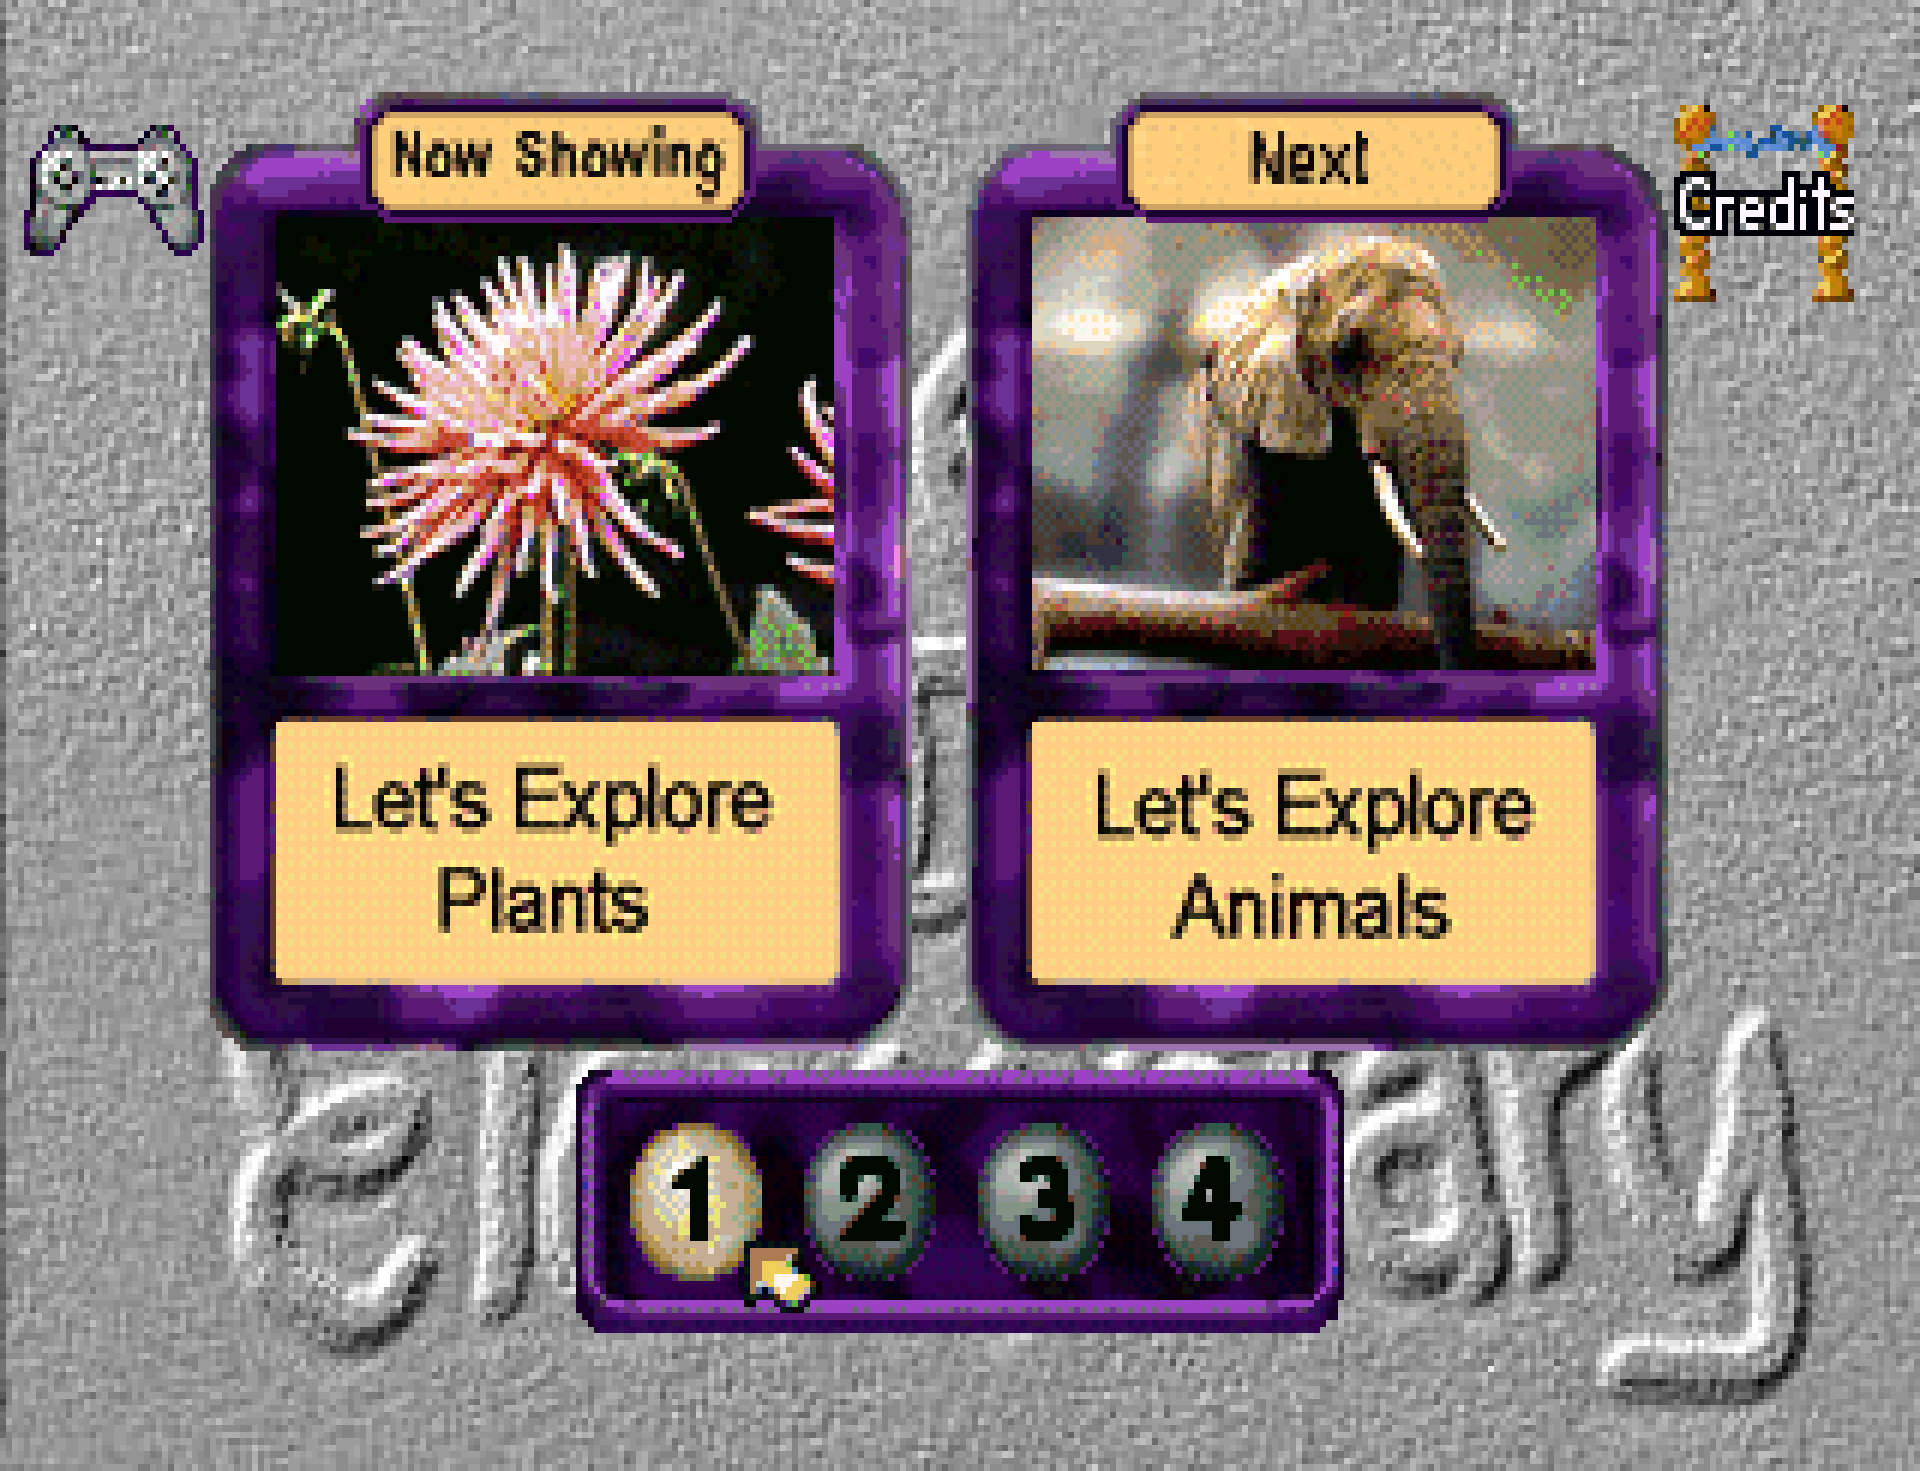
\includegraphics[width=\linewidth]{Games/ScienceIsElementary/Images/ScienceIsElementary1Image1.png}
        \caption{Science Is Elementary 1 - Screenshot 1}
    \end{subfigure}
    \begin{subfigure}{0.45\textwidth}
        \centering
        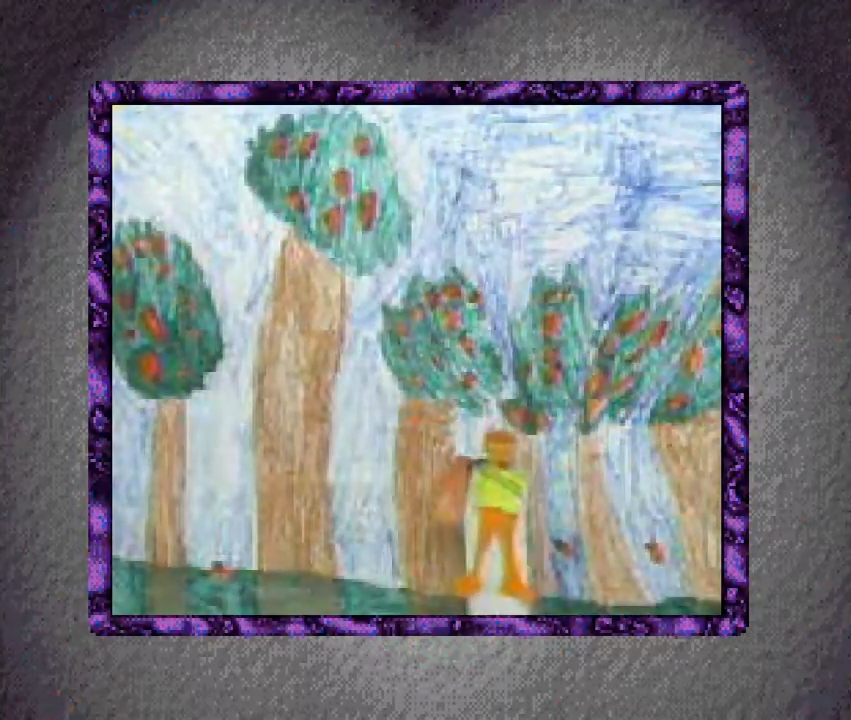
\includegraphics[width=\linewidth]{Games/ScienceIsElementary/Images/ScienceIsElementary1Image2.png}
        \caption{Science Is Elementary 1 - Screenshot 2}
    \end{subfigure}

    \begin{subfigure}{0.45\textwidth}
        \centering
        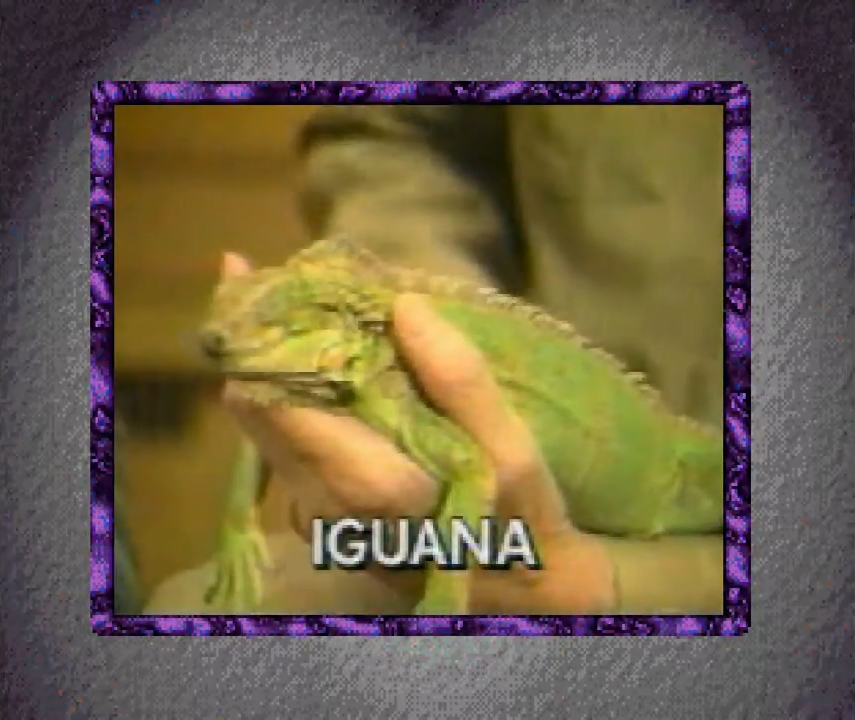
\includegraphics[width=\linewidth]{Games/ScienceIsElementary/Images/ScienceIsElementary1Image3.png}
        \caption{Science Is Elementary 1 - Screenshot 3}
    \end{subfigure}
    \begin{subfigure}{0.45\textwidth}
        \centering
        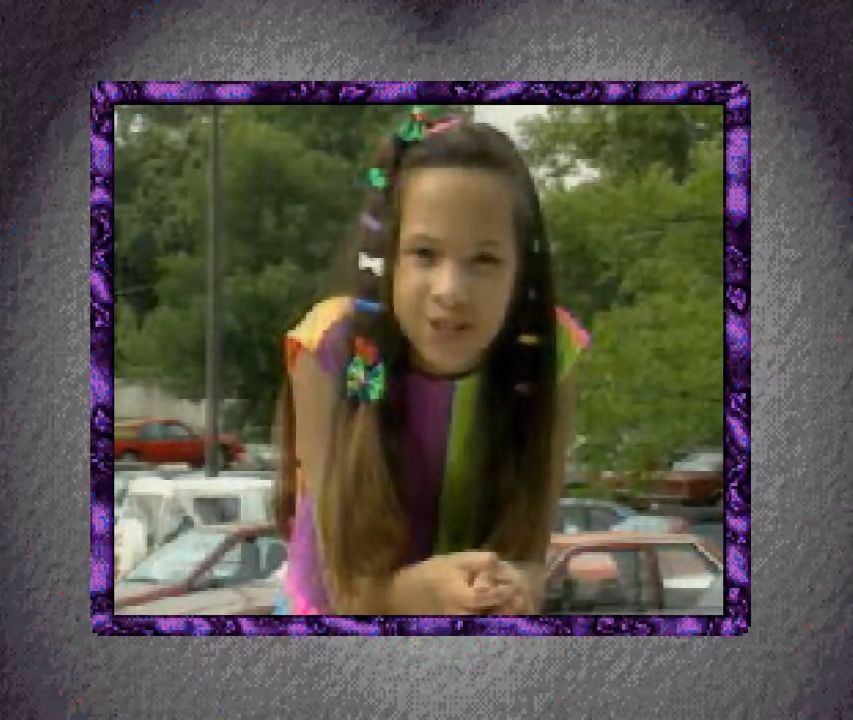
\includegraphics[width=\linewidth]{Games/ScienceIsElementary/Images/ScienceIsElementary1Image4.png}
        \caption{Science Is Elementary 1 - Screenshot 4}
    \end{subfigure}
    \caption{Screenshots from Science Is Elementary 1}
\end{figure}